% !TeX encoding = UTF-8
% !TeX program = pdflatex
% !TeX spellcheck = en_US
\documentclass[binding=0.6cm,LaM,oneside]{sapthesis} % LaM for a Laurea Magistrale
\usepackage{microtype}
\usepackage[utf8]{inputenc}
\usepackage{hyperref}
\usepackage{wrapfig}
\usepackage{float}
\usepackage{booktabs}
\usepackage{amsmath}
\usepackage{algorithm}
\usepackage[noend]{algpseudocode}

\makeatletter
\def\BState{\State\hskip-\ALG@thistlm}
\makeatother

\usepackage{lineno}
\modulolinenumbers[5]
\usepackage{graphicx}
\usepackage{booktabs}
\usepackage{amssymb,amsmath,nccmath}
\usepackage{cclicenses}
\usepackage{makecell}
\usepackage{lscape,array}
\newcolumntype{C}[1]{>{\centering\arraybackslash}p{#1}} 
\usepackage[thin, , thinc]{esdiff}
\usepackage{subcaption}
\usepackage{caption}
\usepackage{framed}  
\usepackage{subcaption}
\usepackage[font=small,skip=0pt]{caption}

\PassOptionsToPackage{hyphens}{url}
\hypersetup{
	colorlinks = true, % Colours links instead of ugly boxes
	urlcolor = black, % Colour for external hyperlinks
	linkcolor = black, % Colour of internal links
	citecolor = black % Colour of citations
}

\usepackage{listings}
\usepackage{xcolor}
\usepackage{multirow}


\renewcommand\baselinestretch{1.5}
\colorlet{punct}{red!60!black}
\definecolor{background}{HTML}{EEEEEE}
\definecolor{delim}{RGB}{20,105,176}
\colorlet{numb}{magenta!60!black}

\lstdefinelanguage{json}{
	basicstyle=\normalfont\ttfamily,
	numbers=left,
	numberstyle=\scriptsize,
	stepnumber=1,
	numbersep=8pt,
	showstringspaces=false,
	breaklines=true,
	frame=lines,
	backgroundcolor=\color{background},
	literate=
	*{0}{{{\color{numb}0}}}{1}
	{1}{{{\color{numb}1}}}{1}
	{2}{{{\color{numb}2}}}{1}
	{3}{{{\color{numb}3}}}{1}
	{4}{{{\color{numb}4}}}{1}
	{5}{{{\color{numb}5}}}{1}
	{6}{{{\color{numb}6}}}{1}
	{7}{{{\color{numb}7}}}{1}
	{8}{{{\color{numb}8}}}{1}
	{9}{{{\color{numb}9}}}{1}
	{:}{{{\color{punct}{:}}}}{1}
	{,}{{{\color{punct}{,}}}}{1}
	{\{}{{{\color{delim}{\{}}}}{1}
	{\}}{{{\color{delim}{\}}}}}{1}
	{[}{{{\color{delim}{[}}}}{1}
	{]}{{{\color{delim}{]}}}}{1},
}

\hypersetup{pdftitle={Investigation of static features for improved APT malware identification},pdfauthor={Leonardo Sagratella}}
\title{Investigation of static features for improved APT malware identification}
\author{Leonardo Sagratella}
\IDnumber{1645347}
\course{CyberSecurity}
\courseorganizer{Facoltà di Ingegneria dell'informazione, informatica e statistica}
\AcademicYear{2019/2020}
\copyyear{2020}
\advisor{Prof. Riccardo Lazzeretti}
\coadvisor{Dr. Giuseppe Laurenza}
\authoremail{leonardosagratella@gmail.com}
\begin{document}
	\frontmatter
	\maketitle
	\dedication{Dedicato a\\ me stesso una stelle nascente e molto simpatica\\
	 ma soprattutto alla mia stella e luce, FEDERICO DI MAIO, figlio di GIGGINO DI MAIO nostro ex-premier nonchè padre fondatore del reddito di cittadinanza}
 	\begin{abstract}
		In the last years, a new cyber-threat is spreading fast, it is know as \textit{Advanced Persistent Threat} (APT). An APT is a criminal or a group that aims to penetrate and exflitrate information from high-valuable target. They rely on malware and tools developed for the specific target they want to attack, usually governments, critical infrastructures or big organizations. Their goal is to break into the target's systems and stay undetected as long as possible. Meanwhile, they steal valuable information and try new ways to infect other target's computers. We propose a framework for malware prioritization to detect, among all the new samples that every day researchers find, the one that can be correlated to an APT group. Those samples are dispatched to analysts for further and manual inspection. To make this process as fast as possible we rely only on static features, without the need of executing the sample. We applied different techniques of feature selection to reduce the dataset dimensionality. We trained a \textit{RandomForestClassifier} with the features left and we analyze its performances. In particular, we are interested in precision, we do not want the analysts to waste time on false positives. Overall, we obtained great performances on both precision and accuracy.
	\end{abstract}
	\tableofcontents
	\mainmatter
	\chapter{Introduction}

In the last decades, we are witnessing the constant improvement of technology and its utility in our every-day life. As technology advances, the cyber-threat arises.
Recently the number of malware increased rapidly, in the last quarter of 2017, McAfee discovered 63.4 million new malware \cite{mcafee2018}, the highest of all time. In 2018 and 2019 AvLab reported on average 12.05 million new samples per month \cite{avtest2020}. Among those malware, there is a small group, known as Advanced Persistent Threat (\textbf{APT}), that is threatening and continuously increasing. 

The National Institute of Standards and Technology (\textbf{NIST}) defines the \textbf{Advanced Persistent Threat} as \cite{nistapt} \textit{"An adversary that possesses sophisticated levels of expertise and significant resources which allow it to create opportunities to achieve its objectives by using multiple attack vectors (e.g., cyber, physical, and deception). These objectives typically include establishing and extending footholds within the information technology infrastructure of the targeted organizations for purposes of exfiltrating information, undermining or impeding critical aspects of a mission, program, or organization; or positioning itself to carry out these objectives in the future."}

The term APT refers to an advanced adversary or a group,that aims to attack some critical infrastructure, a government, or an organization. They use unique attack vectors and ad-hoc malware developed for a specific target, to attack systems and exfiltrate valuable information.

To understand better what is an APT, we need to decompose the word: \cite{apt_def}

\textbf{Advanced:} the people behind the attack have an advanced level of expertise, resources, and money. They usually do not use known malware, but they write their malware specific to the target they want. Moreover, they can gather information on the target from the intelligence of their country of origin.

\textbf{Persistent:}  The adversary does not aim to gain access in the most number of system, but rather to have persistent access to the infrastructure. The more time they remain undiscovered in the organization's network infrastructure, the higher are the chances of lateral movement, the greater are the information they can gather. Persistent access is the key to every APT.

\textbf{Threat:} As said before, this is an organized threat, with a strategical vision of what to achieve. It is not an automatic tool that attacks everything trying to gather something. It is a meticulously planned attack that aims to obtain certain information from a given organization. 

In general, APTs aim to higher-value targets like other nations or some big corporations. However, any individual can be a target. FireEye publish a report each year about the new APT campaign, the diagram below states which industry is the most attacked in the last year.\\

\begin{figure}[!h]
	\centering
	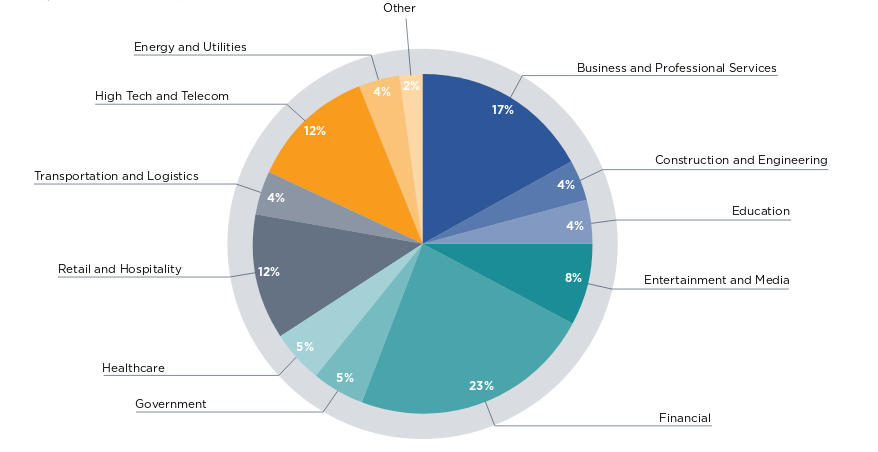
\includegraphics[width=1.0\columnwidth]{graph}
	\caption{Diagram of industry target}
\end{figure}


%A point of particular concern is the retargeting, in the Americas, 63\% of the companies attacked by an APT, are attacked again last year by the same or similar group. In the Asian and Pacific areas, this is even worse, 78\% of the industries are hacked again. \cite{fireeye_mtrends} \\


%\begin{figure}[ht!]
%	\centering
%	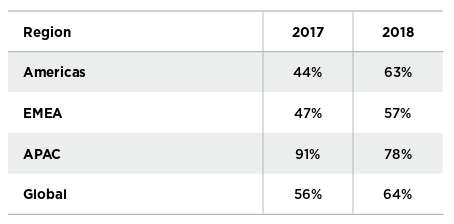
\includegraphics[width=0.5\columnwidth]{retarget}
%	\caption{Retargeting divided by regions}
%\end{figure}

\textit{Advanced persistent threats}, contrary to regular malware, are composed of different phases, each of which has an important role. 

The attack is decomposed into smaller steps, for example, if a group of hackers wants to attack a CEO of a given company, they will not send directly to the CEO a phishing email, because it's likely that he has a complex system of security and they would be detected instantly. 

Instead, the first step would hack a person in the same company with lower permissions that can have minor defense mechanisms, or hack some organization that works with the one we want to attack. Once they got the first computer, they can explore the network infrastructure of the organization, and then decide which action is the best.
They could cover their track from the log system, or locate the data they need or send a phishing email to the CEO from the owned user.

So how does an APT work? Fireeye described their behavior in six steps. \cite{fireeye_anatomy}

\begin{enumerate}
	\item The adversary gains access into the network infrastructure, installing a malware sent through a phishing email or by exploiting some vulnerability.
	\item Once they comprised the network, the malware scans all the infrastructure looking for other entry points or weaknesses. It can communicate with a Command \& Control server (C\&C) to receive new instructions or to send information.
	\item The malware typically establishes additional points of compromise to ensure that the attack can continue even if a position is closed.
	\item Once the attackers have a reliable connection to the network, they start dumping data such as usernames and passwords, to gain credentials.
	
	\item The malware sends the data to a server where the attackers can receive the information. Now the network is breached.
	
	\item The malware tries to cover its tracks cleaning the log system, but the network is still compromised so the adversary can enter again if they are not detected.
\end{enumerate}

Since APTs targets Critical Infrastructures, Governments, Organizations, they are mighty and critical. Analysts and researchers work every day to dissect and analyze malware. However, due to their constant increase, researchers can no more handle all of them. We proposed a prioritization system to dispatch to analysts only the samples that can be related to an APT campaign. Our system uses static features from code analysis to train a model to classify each malware.

In Chapter \ref{ch:rel-works}, we analyze all the paper that we use to start this thesis. We talk about a novel framework for APT malware prioritization proposed by Laurenza et al. In the next section, we analyze the work made by Caliskan et al., where they show how it is still possible to de-anonymize different programmers just relying on executable files. The last work of Dubyk shows the usage of an undocumented section of the PE header, Rich Header, in malware classification.

Chapter \ref{ch:rel-works} introduces the preliminaries notions needed for the comprehension of this thesis. It focuses on Reverse Engineering (\textbf{RE}) and shows which documents are useful for an analyst in code analysis. Then we present the state-of-the-art of RE tools, why we chose Ghidra, and all its functionality useful for code analysis. Furthermore, we present the tools used for machine-learning tasks.

Chapter \ref{ch:feat-cre} focuses on how we extracted features from the dataset using Ghidra. We shows the different block of features proposed in Chapter \ref{ch:prelim}, and for each them, we present the type of features selected and how we accomplished the task.

Chapter \ref{ch:classif} introduces all the machine-learning models and techniques used. It presents the \textit{RandomForest} and \textit{XGBoost} classifier, the problem of validating results obtained from a model. Moreover, we present the different techniques for feature selection used to shrink our feature vector.

Chapter \ref{ch:disc} comprehends all the tests we made to evaluate our models. We present in detail the results of feature selection and how we chose the best for our purpose.
Furthermore, we analyzed the performances of the two models.

In Chapter \ref{ch:future} we show the future works we could make to improve this thesis. 
	\chapter{Related works}
\section{APT triage}
Laurenza et al. show that it is possible to help an analyst lightening the number of samples to analyze. The main idea is to process all the executables, extract some features, and then classify them to determine if they belong or not to a possible APT campaign. The analyst can then analyze only the suspected files that can be related to some APT. Unfortunately, this work has some drawbacks. First of all, it is possible to identify only samples correlated to a known APT campaign, if the sample belongs to a new never investigated APT, then it is impossible to detect it. Furthermore, even if the executable belongs to a known APT, there is no guarantee that the classifier detects it because it just relies on information present in the header of the file. The malware writer can hijack that information to mislead the model. \\


The dataset used by Laurenza et al. is \textbf{dAPTaset}, a public database that collects data related to APTs from existing public sources through a semi-automatic methodology and produces an exhaustive dataset. Unfortunately, the dataset is not big enough and is not perfectly balanced. It contains only 2086 samples because there are not many samples belonging to an APT campaign. Instead, the majority of public analyzed samples are just malware.

\section{De-anonymizing Programmers from Executable Binaries}
In this paper, Caliskan et al. presented their approach to de-anonymize different programmers from their compiled programs. They used a dataset of executables from Google Code Jam, and they show that even after compilation the author fingerprints persist in the code, and it is still possible to de-anonymize them.\\

Their approach was to extract distinct blocks of features with different tools and then analyze them to determine the best ones to describe the stylistic fingerprint of the authors precisely. Firstly,  with a disassembler is possible to disassemble the binary and to obtain the low-level features in assembly code.

Then with a decompiler, they extracted the \textbf{Control Flow Graph} and the \textbf{Abstract Syntax Tree}. They determine the stylistics features from those four documents.
\\
In particular, the tools used are \textbf{ndisasm} \textbf{radare2} disassembler for the disassembled code and the Control Flow Graph; \textbf{Hexray} decompiler for the pseudocode, which is passed as input to \textbf{Joern}, a C fuzzy parser, to produce the  \textbf{Abstract Syntax Tree}.\\

They used different types of features selection techniques to reduce the number of features to only 53. They trained a RandomForest Classifier with the dataset created to de-anonymize the authors correctly. \\

This paper is an entry point for our work, and we tried to apply the same approach to the apt triage problem. However, the tools used by Caliskan et al. are outdated and no more maintained, so we decided to use the novel open-source tool ghidra to write the script and extract the information we want. In this way, we significantly reduced the amount of time for feature extraction.



\section{Rich Header}
\textbf{da scrivere sunto del lavoro su rich header}
\cite{dubyk2019sans}

\section{Advanced Persistent Threat}

APT stands for Advanced Persistent Threat, a kind of sophisticated attack which requires an advanced level of expertise and aims to remain persistent on the attacked infrastructure.

The term APT can refer to a persistent attack with a specific target, or it can refer to the group that organized the attack, sometimes the group is affiliated with some sovereign state.
\\

To understand better what is an APT, we need to decompose the word: 

\textbf{Advanced:} the people behind the attack have an advanced level of expertise, resources, and money. They usually do not use known malware, but they write their malware specific to the target they want. Moreover, they can gather information on the target from the intelligence of their country of origin.

\textbf{Persistent:}  The adversary does not aim to gain access in the most number of system, but rather to have persistent access to the infrastructure. The more time they remain undiscovered in the organization's network infrastructure, the higher are the chances of lateral movement, the greater are the information they can gather. Persistent access is the key to every APT.

\textbf{Threat:} As said before, this is an organized threat, with a strategical vision of what to achieve. It is not an automatic tool that attacks everything trying to gather something. It is a meticulously planned attack that aims to obtain certain information from a given organization. \cite{apt_def}
\\

In general, APTs aim to higher-value targets like other nations or some big corporations. However, any individual can be a target. FireEye publish a report each year about the new APT campaign, the diagram below states which industry is the most attacked in the last year.\\

\begin{figure}[!h]
	\centering
	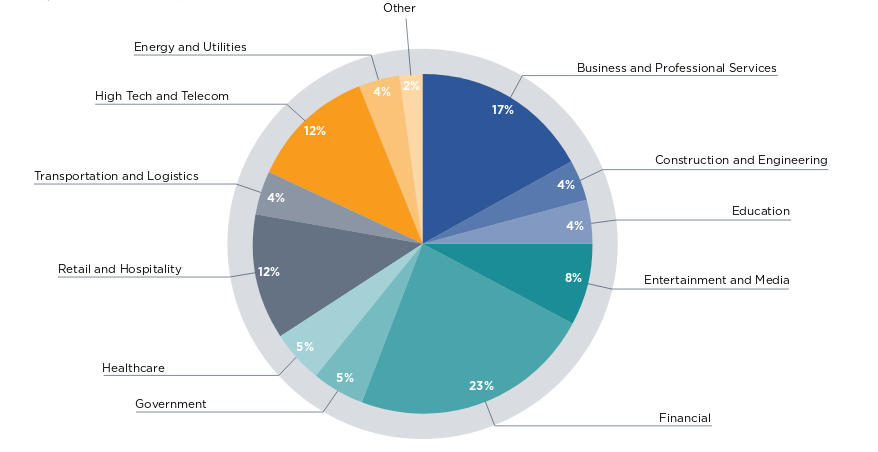
\includegraphics[width=1.0\columnwidth]{graph}
	\caption{Diagram of industry target}
\end{figure}

A point of particular concern is the retargeting, in the Americas, 63\% of the companies attacked by an APT, are attacked again last year by the same or similar group. In the Asian and Pacific areas, this is even worse, 78\% of the industries are hacked again. \cite{fireeye_mtrends} \\


\begin{figure}[ht!]
	\centering
	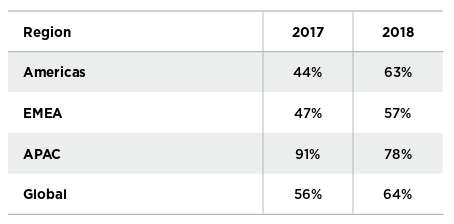
\includegraphics[width=0.5\columnwidth]{retarget}
	\caption{Retargeting divided by regions}
\end{figure}

Advanced persistent threats, contrary to regular malware, are composed of different phases, each of which has an important role. 

The attack is decomposed into smaller steps, for example, if a group of hackers wants to attack a CEO of a given company, they will not send directly to the CEO a phishing email, because it's likely that he has a complex system of security and they would be detected instantly. 

Instead, the first step would hack a person in the same company with lower permissions that can have minor defense mechanisms. Once they got the first computer, they can explore the network infrastructure of the organization, and then decide which action is the best.
They could cover their track from the log system, or locate the data they need or send a phishing email to the CEO from the owned user.\\

So how does an APT work? Fireeye described their behavior in six steps. \cite{fireeye_anatomy}


\begin{enumerate}
	\item The adversary gains access into the network infrastructure, installing a malware sent through a phishing email or by exploiting some vulnerability.
	\item Once they comprised the network, the malware scans all the infrastructure looking for other entry points or weaknesses. It can communicate with a Command \& Control server (C\&C) to receive new instructions or to send information.
	\item The malware typically establishes additional points of compromise to ensure that the attack can continue even if a position is closed.
	\item Once the attackers have a reliable connection to the network, they start dumping data such as usernames and passwords, to gain credentials.
	
	\item The malware sends the data to a server where the attackers can receive the information. Now the network is breached.
	
	\item The malware tries to cover its tracks cleaning the log system, but the network is still compromised so the adversary can enter again if they are not detected.
	
\end{enumerate}
	\chapter{Preliminaries}
\section{Advanced Persistent Threat}

APT stands for Advanced Persistent Threat, a kind of sophisticated attack which requires an advanced level of expertise and aims to remain persistent on the attacked infrastructure.

The term APT can refer to a persistent attack with a specific target, or it can refer to the group that organized the attack, sometimes the group is affiliated with some sovereign state.
\\

To understand better what is an APT, we need to decompose the word: 

\textbf{Advanced:} the people behind the attack have an advanced level of expertise, resources, and money. They usually do not use known malware, but they write their malware specific to the target they want. Moreover, they can gather information on the target from the intelligence of their country of origin.

\textbf{Persistent:}  The adversary does not aim to gain access in the most number of system, but rather to have persistent access to the infrastructure. The more time they remain undiscovered in the organization's network infrastructure, the higher are the chances of lateral movement, the greater are the information they can gather. Persistent access is the key to every APT.

\textbf{Threat:} As said before, this is an organized threat, with a strategical vision of what to achieve. It is not an automatic tool that attacks everything trying to gather something. It is a meticulously planned attack that aims to obtain certain information from a given organization. \cite{apt_def}
\\

In general, APTs aim to higher-value targets like other nations or some big corporations. However, any individual can be a target. FireEye publish a report each year about the new APT campaign, the diagram below states which industry is the most attacked in the last year.\\

\begin{figure}[!h]
	\centering
	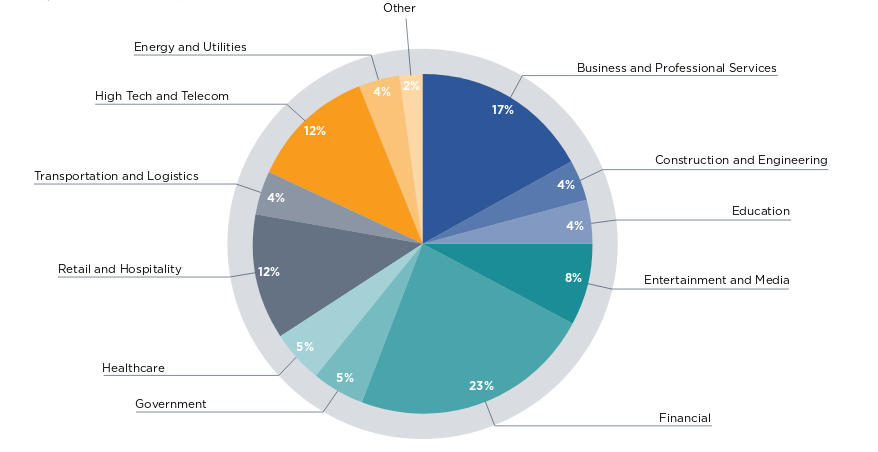
\includegraphics[width=1.0\columnwidth]{graph}
	\caption{Diagram of industry target}
\end{figure}

A point of particular concern is the retargeting, in the Americas, 63\% of the companies attacked by an APT, are attacked again last year by the same or similar group. In the Asian and Pacific areas, this is even worse, 78\% of the industries are hacked again. \cite{fireeye_mtrends} \\


\begin{figure}[ht!]
	\centering
	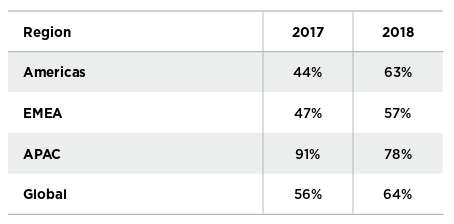
\includegraphics[width=0.5\columnwidth]{retarget}
	\caption{Retargeting divided by regions}
\end{figure}

Advanced persistent threats, contrary to regular malware, are composed of different phases, each of which has an important role. 

The attack is decomposed into smaller steps, for example, if a group of hackers wants to attack a CEO of a given company, they will not send directly to the CEO a phishing email, because it's likely that he has a complex system of security and they would be detected instantly. 

Instead, the first step would hack a person in the same company with lower permissions that can have minor defense mechanisms. Once they got the first computer, they can explore the network infrastructure of the organization, and then decide which action is the best.
They could cover their track from the log system, or locate the data they need or send a phishing email to the CEO from the owned user.\\

So how does an APT work? Fireeye described their behavior in six steps. \cite{fireeye_anatomy}


\begin{enumerate}
	\item The adversary gains access into the network infrastructure, installing a malware sent through a phishing email or by exploiting some vulnerability.
	\item Once they comprised the network, the malware scans all the infrastructure looking for other entry points or weaknesses. It can communicate with a Command \& Control server (C\&C) to receive new instructions or to send information.
	\item The malware typically establishes additional points of compromise to ensure that the attack can continue even if a position is closed.
	\item Once the attackers have a reliable connection to the network, they start dumping data such as usernames and passwords, to gain credentials.
	
	\item The malware sends the data to a server where the attackers can receive the information. Now the network is breached.
	
	\item The malware tries to cover its tracks cleaning the log system, but the network is still compromised so the adversary can enter again if they are not detected.
	
\end{enumerate}

\section{Reverse Enigneering}

Reverse engineering is the process of decomposing a human-made object to understand the underlying architecture, how it works, or to extract some information from it. This process can be applied in various fields, such as computer science, electronic, mechanical, or chemical \cite{eilam2011reversing}.

We focus on reverse engineering applied to computer science. 
\\

The Institute of Electrical and Electronics Engineers (\textbf{IEEE}) states that reverse engineering is \textit{"The process of analyzing a subject system to identify the system's components and their interrelationships, and to create representations of the system in another form or at a higher level of abstraction."}, where the \textit{"subject system"} is referred to the software development \cite{chikofsky1990reverse}. 

When somebody writes a software, he writes it with a language that is understandable by a human, for example, C or Java.  But the computer can not read it, so the programmer needs to compile the source code to let the computer understand what the software should do. 

The compiling process is the process of translating the source code into a language understandable by a computer. But once the program is compiled, a human can no more read it, unless it has the corresponding source code. 

If we want to understand a binary executable, but its source code is not available, we need to reverse it. There are different techniques of reversing for binary executable: disassembling the binary using a disassembler, decompiling the binary with a decompiler, or analyzing the information exchanged with a bus sniffer or a packet sniffer.


\subsection{Disassembly code}

Assembly language is a low-level programming language that has a substantial correspondence with the architecture's machine code. The program used to convert the assembly instruction to machine code instruction is called assembler. Since the assembly depends on the machine code, there is an assembly language, with its assembler, for each architecture.

With a disassembler, it is possible to revert the actions made by the assembler, so it's possible to translate machine code instruction to assembly language. The output code is formatted for human readability.

\subsection{Decompiler?}

\subsection{Control Flow Graph}

\subsection{Cyclomatic Complexity}



\section{Ghidra}
Ghidra is an open-source tool for Reverse Engineering developed and by the National Security Agency (NSA). It helps analyze malicious code and malware like viruses, and can give cybersecurity professionals a better understanding of potential vulnerabilities in their networks and systems \cite{ghidra}
\begin{wrapfigure}{L}{0.35\textwidth}
	\centering
	
\includegraphics[width=0.35\textwidth]{ghidra}
	
\end{wrapfigure}


Usually, reverse engineering is the process of analyzing something to understand how it works. In the case of a program written in Java or C or C++, the code will be readable by a human but not bt a computer. It needs to be compiled in a language understandable by the network, but once it is compiled, we can no more read it. \\

To understand how the program works, we need a toolkit to take it apart, and this is what Ghidra does. There are a lot of tools in the market that can do the same thing, in different ways, some of them are open-source and free, other you need to pay a license. 

We choose to use Ghidra because it is free, and it offers the possibility of writing scripts to run against the binaries analyzed. In this way, we extracted all the necessary information automatically from the APT binaries.

\subsection{PCode}
\textbf{la parte che segue è tutta da riscrivere in quanto CTRL+C CTRL+V diretto da Ghidra doc} \cite{ghidra_pcode}
titolo da cambiare\\

P-code is a register transfer language designed for reverse engineering applications. The language is general enough to model the behavior of many different processors. By modeling in this way, the analysis of different processors is put into a common framework, facilitating the development of retargetable analysis algorithms and applications.

Fundamentally, p-code works by translating individual processor instructions into a sequence of p-code operations that take parts of the processor state as input and output variables (varnodes). The set of unique p-code operations (distinguished by opcode) comprise a fairly tight set of the arithmetic and logical actions performed by general purpose processors. The direct translation of instructions into these operations is referred to as raw p-code. Raw p-code can be used to directly emulate instruction execution and generally follows the same control-flow, although it may add some of its own internal control-flow. The subset of opcodes that can occur in raw p-code is described in the section called “P-Code Operation Reference” and in the section called “Pseudo P-CODE Operations”, making up the bulk of this document.

P-code is designed specifically to facilitate the construction of data-flow graphs for follow-on analysis of disassembled instructions. Varnodes and p-code operators can be thought of explicitly as nodes in these graphs. Generation of raw p-code is a necessary first step in graph construction, but additional steps are required, which introduces some new opcodes. Two of these, MULTIEQUAL and INDIRECT, are specific to the graph construction process, but other opcodes can be introduced during subsequent analysis and transformation of a graph and help hold recovered data-type relationships. All of the new opcodes are described in the section called “Additional P-CODE Operations”, none of which can occur in the original raw p-code translation. Finally, a few of the p-code operators, CALL, CALLIND, and RETURN, may have their input and output varnodes changed during analysis so that they no longer match their raw p-code form.
\subsection{Address Space}
The address space for p-code is a generalization of RAM. It is defined simply as an indexed sequence of bytes that can be read and written by the p-code operations. For a specific byte, the unique index that labels it is the byte's address. An address space has a name to identify it, a size that indicates the number of distinct indices into the space, and an endianess associated with it that indicates how integers and other multi-byte values are encoded into the space. A typical processor will have a ram space, to model memory accessible via its main data bus, and a register space for modeling the processor's general purpose registers. Any data that a processor manipulates must be in some address space. The specification for a processor is free to define as many address spaces as it needs. There is always a special address space, called a constant address space, which is used to encode any constant values needed for p-code operations. Systems generating p-code also generally use a dedicated temporary space, which can be viewed as a bottomless source of temporary registers. These are used to hold intermediate values when modeling instruction behavior.

P-code specifications allow the addressable unit of an address space to be bigger than just a byte. Each address space has a wordsize attribute that can be set to indicate the number of bytes in a unit. A wordsize which is bigger than one makes little difference to the representation of p-code. All the offsets into an address space are still represented internally as a byte offset. The only exceptions are the LOAD and STORE p-code operations. These operations read a pointer offset that must be scaled properly to get the right byte offset when dereferencing the pointer. The wordsize attribute has no effect on any of the other p-code operations. 

\subsection{Varnode}
A varnode is a generalization of either a register or a memory location. It is represented by the formal triple: an address space, an offset into the space, and a size. Intuitively, a varnode is a contiguous sequence of bytes in some address space that can be treated as a single value. All manipulation of data by p-code operations occurs on varnodes.

Varnodes by themselves are just a contiguous chunk of bytes, identified by their address and size, and they have no type. The p-code operations however can force one of three type interpretations on the varnodes: integer, boolean, and floating-point.

Operations that manipulate integers always interpret a varnode as a twos-complement encoding using the endianess associated with the address space containing the varnode.
A varnode being used as a boolean value is assumed to be a single byte that can only take the value 0, for false, and 1, for true.
Floating-point operations use the encoding expected by the processor being modeled, which varies depending on the size of the varnode. For most processors, these encodings are described by the IEEE 754 standard, but other encodings are possible in principle.

If a varnode is specified as an offset into the constant address space, that offset is interpreted as a constant, or immediate value, in any p-code operation that uses that varnode. The size of the varnode, in this case, can be treated as the size or precision available for the encoding of the constant. As with other varnodes, constants only have a type forced on them by the p-code operations that use them. 

\subsection{Pcode Operations}
A p-code operation is the analog of a machine instruction. All p-code operations have the same basic format internally. They all take one or more varnodes as input and optionally produce a single output varnode. The action of the operation is determined by its opcode. For almost all p-code operations, only the output varnode can have its value modified; there are no indirect effects of the operation. The only possible exceptions are pseudo operations, see the section called “Pseudo P-CODE Operations”, which are sometimes necessary when there is incomplete knowledge of an instruction's behavior.

All p-code operations are associated with the address of the original processor instruction they were translated from. For a single instruction, a 1-up counter, starting at zero, is used to enumerate the multiple p-code operations involved in its translation. The address and counter as a pair are referred to as the p-code op's unique sequence number. Control-flow of p-code operations generally follows sequence number order. When execution of all p-code for one instruction is completed, if the instruction has fall-through semantics, p-code control-flow picks up with the first p-code operation in sequence corresponding to the instruction at the fall-through address. Similarly, if a p-code operation results in a control-flow branch, the first p-code operation in sequence executes at the destination address.


\section{Scikit-learn}
Scikit-learn is a Python module integrating a wide range of state-of-the-art machine learning algorithms for medium-scale supervised and unsupervised problems. 

It is open-source, commercially usable, and contains many modern machine learning algorithms for classification, regression, clustering, feature extraction, and optimization.
For this reason, Scikit-Learn is often the first tool in a Data Scientists toolkit for machine learning of incoming data sets. \cite{scikit-learn}
\section{Jupyter Notebook}



	\chapter{Features Creation}

When we decided which features could be the most representative for our model, we choose to use only static features. Extracting only static features usually do not require too much time, and there is no need for expensive virtualized systems. In the dynamic analysis, the sample has to be executed in a controlled environment to analyze its behavior. 

Since we want to boost up the work made by Laurenza et al., we choose to continue their path of using only static features, but we added novel features from code analysis.  We are looking for a framework fast and efficient, that can analyze lots of sample without being resource expensive.

At first, we tried to replicate the work done by Caliskan et al., but we found that most of the tools used depend on software no more maintained. Some of those tools do not work as expected, and others were slow in processing files. To simplify as much as possible the process of analyzing executables, we decided to use only Ghidra as software for extracting features.

Ghidra comes with a headless analyzer, which analyzes and runs scripts on the given sample. The headless version can run in any server, even without a desktop environment. So we built up a virtual machine in the Sapienza network and installed Ghidra there.  Unfortunately, Ghidra's documentation is not exhaustive since it was released less than a year ago. The hardest part was understanding Ghidra's APIs and how to exploit them for our purpose. The already made scripts were useful for our task because they contain many approaches for extracting data. \\



The following sections will cover the blocks of features extracted, explaining the procedure used to accomplish this task.

\section{Dataset file format}
The choice of the format used for storing our dataset was crucial.
We decided to save a single file for each sample into a \texttt{.csv } file. We calculated the md5 of each sample and we used it to find the related APT campaign in the dAPTaset. Each \texttt{.csv} file contains a column named md5, a column name apt, and \texttt{n} columns corresponding to the features vector of the sample. During the classification phase the md5s are stripped out from the dataset and the apt column is the label of each sample.

To generate the dataset with all the features vectors of all the samples, we tried different approaches. 

The first one was to merge all the \texttt{.csv} files into a single big \texttt{.csv}. Unfortunately, the more features we extracted, the more significant was the dimensionality of our dataset.  When it comes to reading into python, pandas was very slow in both reading and processing the files.

A valid alternative to pandas is \textit{Dask}, a flexible parallel computing library for analytics, that integrates with \textit{pandas},  \textit{numpy}, and \textit{scikit}. However, the dask-ml package lacks some functionalities for the cross-validation and random forest model. Furthermore, It was still slow in reading bigger files, so we decided to find another solution to speed up the process.

In the end, we decided to store our dataset into a \textit{Hierarchical Data Format} (\textbf{HDF5}) designed to store and organize large amounts of data. This format comes with a cost, the files are much bigger, but we drastically improved the speed of reading and processing the dataset.


\section{Disassembled features}

The extraction of disassembled code was an easy and fast task. The documentation provides all the information on how to correctly use the disassembler. We wrote a script that extracts the disassembled code for each function and stores it into a \texttt{.dis} file. The script creates a folder for each sample and stores inside the disassembled code.

From the disassembled code, we extracted 5 kinds of various features:
\begin{itemize}
	\item{Line unigrams}
	\item{Disassemble unigrams}
	\item{Disassemble bigrams}
	\item{Instruction only unigrams}
	\item{Instruction only bigrams}
\end{itemize}

First of all, we stripped out all the hexadecimal and numbers, replacing the regex \texttt{"$\backslash$d+"} with the word \texttt{"number"}, and \texttt{"0[xX][0-9a-fA-F]+"} with the word \texttt{"hexadecimal"}. Stripping the numbers and hexadecimal reduced the possibility of overfitting because some numbers may be unique, and that would create a useless feature.


\subsection{Line unigram}
The first block of features is the whole line unigram, we split the disassembled code of each function on the new-line character and then count all the occurrences of different line instructions. We stripped out all the commas because, in the beginning, we saved the dataset to \texttt{.csv} with comma as a separator. For example, the features generated from the function f in Table \ref{tab:function_f} are shown in Table \ref{tab:line_unigrams}

\begin{table}[!htb]
\begin{minipage}{.5\linewidth}
	\centering
	
	\caption{Code for function f}
	\label{tab:function_f}
	
	\medskip
	
	\begin{tabular}{ l } 
		\toprule
		\texttt{push ebx} \\
		\texttt{mov eax, 1}\\
		\texttt{cmp ebx, eax}\\
		\texttt{jle 0xDEADBEEF}\\
		\texttt{add eax, 1}\\
		\texttt{cmp ebx, eax}\\
		\texttt{jle 0xBACADDAC}\\
		\texttt{mov eax, 0x400231BC}\\
		\texttt{call eax}\\
		\texttt{ret}\\
	
		
		\bottomrule
	\end{tabular}
\end{minipage}\hfill
\begin{minipage}{.5\linewidth}
	\centering
	
	\caption{Feature vector of line unigrams}
	\label{tab:line_unigrams}
	
	\medskip
	
	\begin{tabular}{  lr } 
		\toprule
		\makecell{ Feature }  &  Value \\   
		
		\midrule push ebx       & 1         \\
		\texttt{mov eax,number} & 1                  \\ 
		\texttt{cmp ebx,eax }   & 2                  \\ 
		\texttt{add ebx, number}     & 2                  \\ 
		\texttt{jle hex }       & 2                  \\
		\texttt{mov eax, hexadecimal} & 1\\ 
		\texttt{call eax}       & 1                  \\
		\texttt{ret} & 1\\
		\bottomrule
	\end{tabular}
\end{minipage}
\end{table}


\subsection{Disassemble unigrams and bigrams}
For this block of features, we split the entire line in instruction, eventual registers, or numbers. Firstly, we split the line on the first space, then if the second half of the string still contains data, we split for all the commas to get the single registers/numbers. The line \texttt{"mov eax, 0x12"} would be split in the following array: \texttt{["mov", "eax", "hexadecimal"]} . As before, we counted the occurrences of every word in the file. 

For the unigram files, we only considered as a feature every word we would obtain after splitting the string. For the bigram files, instead, we considered as a feature the pair of words in the file. 

Furthermore, we added a start token (\texttt{"<s>"}) before the first instruction of every function, and an end token (\texttt{"</s>"}) after the last instruction. We concatenate the first and second element of the bigram with the the string \texttt{"=>"} The features generated from the same disassembled code are presented in Table \ref{tab:dis_uni} and \ref{tab:dis_big}.

\begin{table}[!htb]
	\begin{minipage}{.5\linewidth}
		\centering
		
		\caption{Disassemble unigrams}
		\label{tab:dis_uni}
		
		\medskip
		
		\begin{tabular}{  lr } 
			\toprule
			\makecell{ Feature }  &  Value \\   
			
			\midrule 
			\texttt{push} & 1	\\
			\texttt{ebx} & 3\\
			\texttt{mov} & 2\\
			\texttt{eax} & 6\\
			\texttt{number} & 2\\
			\texttt{cmp} & 2\\
			\texttt{jle} & 2\\
			\texttt{hex} & 3\\
			\texttt{add} & 1\\
			\texttt{call} & 1\\
			\texttt{ret} & 1\\
			\bottomrule
		\end{tabular}
	\end{minipage}\hfill
	\begin{minipage}{.5\linewidth}
		\centering
		
		\caption{Disassemble bigrams}
		\label{tab:dis_big}
		
		\medskip
		
		\begin{tabular}{  lr } 
			\toprule
			\makecell{ Feature }  &  Value \\   
			
			\midrule 
			\texttt{<s>=>push} & 1	\\
			\texttt{push=>ebx} & 1\\
			\texttt{ebx=>mov} & 1\\
			\texttt{mov=>eax} & 2\\
			\texttt{eax=>num} & 2\\
			\texttt{num=>cmp} & 2\\
			\texttt{cmp=>ebx} & 2\\
			\texttt{ebx=>eax} & 2\\
			\texttt{eax=>jle} & 2\\
			\texttt{jle=>hex} & 2\\
			\texttt{hex=>add} & 1\\
			\texttt{add=>eax} & 1\\
			\texttt{hex=>mov} & 1\\
			\texttt{eax=>hex} & 1\\
			\texttt{hex=>call} & 1\\
			\texttt{call=>hex} & 1\\
			\texttt{hex=>ret} & 1\\
			\texttt{ret=></s>} & 1\\
			\bottomrule
		\end{tabular}
	\end{minipage}
\end{table}


\subsection{Instruction only unigrams and bigrams}
For the last block of features, we decided to study only the frequency of the different instructions in the code, without considering the registry. As before in the bigrams, we added a start and an end token to avoid linking two instructions from different functions. The features from the previous example would be:

\begin{table}[!htb]
	\begin{minipage}{.5\linewidth}
		\centering
		
		\caption{Instruction only unigrams}
		\label{tab:instr_uni}
		
		\medskip
		
		\begin{tabular}{  lr } 
			\toprule
			\makecell{ Feature }  &  Value \\   
			
			\midrule 
			\texttt{push} & 1	\\
			\texttt{mov} & 2\\
			\texttt{cmp} & 2\\
			\texttt{jle} & 2\\
			\texttt{add} & 1\\
			\texttt{call} & 1\\
			\texttt{ret} & 1\\
			\bottomrule
		\end{tabular}
	\end{minipage}\hfill
	\begin{minipage}{.5\linewidth}
		\centering
		
		\caption{Instruction only bigrams}
		\label{tab:instr_big}
		
		\medskip
		
		\begin{tabular}{  lr } 
			\toprule
			\makecell{ Feature }  &  Value \\   
			
			\midrule 
			\texttt{<s>=>push} & 1	\\
			\texttt{push=>mov} & 1\\
			\texttt{mov=>cmp} & 1\\
			\texttt{cmp=>jle} & 2\\
			\texttt{jle=>add} & 1\\
			\texttt{add=>cmp} & 1\\
			\texttt{jle=>mov} & 1\\
			\texttt{mov=>call} & 1\\
			\texttt{call=>ret} & 1\\
			\texttt{ret=></s>} & 1\\
			\bottomrule
		\end{tabular}
	\end{minipage}
\end{table}

\section{Control Flow Graph features}
For \textit{Control Flow Graph} features we proceed by creating a \texttt{.json} file with all the information gathered from the Decompiler as explained in Subsection \ref{subsec:cfg_ghidra}.

From the CFG files, we extracted three kinds of features:
\begin{itemize}
	\item {Control Flow Graph unigrams complete}
	\item {Control Flow Graph unigrams Pcode only}
	\item {Control Flow Graph bigrams Pcode only}
\end{itemize}

\subsection{Control Flow Graph unigrams complete}
This first set of features contains the unigrams of the complete Pcode representation.
For each sample we extract, from the corresponding \texttt{.json} file, all the pcodes in that function. We consider as a feature every unique combination of pcodes with input and output varnodes.
The key for each feature is the concatenation of the PcodeOP, the input and output varnodes. In particular, we construct the key as follow:
\texttt{PCodeOP\_nodeoutput\#nodeinput*count} of nodes.

So the key of the example in \ref{lst:jsonpcode} is \texttt{call\_ram\#const*2}.

\clearpage
\begin{lstlisting}[language=json,firstnumber=1,caption={Example of .json format with PCode},label={lst:jsonpcode}]
{
"pcodes": [
	{
	"code": "CALL",
	"varnode_in": ["ram","const"],
	"count": 2 
	}]
}
\end{lstlisting}

We counted the occurrences of each key and we built our dataset.

\subsection{Control Flow Graph Pcode only unigrams and bigrams}

These two sets of features contain the unigrams and bigrams of the pcode only. We built the key using only the pcode operator, and then counted the occurrences. For the bigrams, we concatenated as before the key with the string =>.

\subsection{Cyclomatic Complexity}

To calculate the Cyclomatic Complexity of a given function, we used the class from Ghidra's API \texttt{CyclomaticComplexity}. The function has a method that returns the complexity of the given function. We saved for every function of each sample its complexity. 

Then, for each sample, we calculated \textit{maximum}, \textit{mean}, and \textit{standard variation} of the complexity of all the functions, and used those as features.

\subsection{Standard Library}

One primary task of reverse engineering binary code is to identify library code. Since what the library code does is often known, it is of no interest to an analyst. Hex-Rays has developed the IDA FLIRT signatures to tackle the problem. 

Function ID is Ghidra's function signature system. Unfortunately, Ghidra has very few Function ID datasets. There is only function identification for the Visual Studio supplied libraries. Ghidra's Function ID allows identifying functions based on hashing the masked function bytes automatically.\cite{ghidra_fid}\\

We exploit this functionality to determine which of the functions belongs to a standard library and added a boolean field in the \texttt{.json} file, indicating whether that function is or not a standard known function. Then we calculated the number of standard functions in the given sample and use it as a feature.

\section{Rich Header features}
We used the script in the paper \cite{dubyk2019sans} to calculate the rich hash and pv for each of the samples. Sadly, as pointed out in the paper, not every binary is compiled with the rich header; in fact, only 1669 samples out of 2086 have it. 

The script extracts the \texttt{productID}, the \texttt{productVersion}, and \texttt{productCount}, we concatenated those numbers with a dash \texttt{"-"} to create a key and set 1 if the sample contains the previous key, 0 otherwise.

As suggested by the author, we also calculated a new feature vector without using the productCount field, that is the field that varies the most between all the samples.

\section{Total features}
Table \ref{tab:num_feat} shows the number of features of each type, with a total number of \textbf{218012} features.

\begin{table}[!htb]
		\centering
		\caption{Number of features of each type}
		\label{tab:num_feat}
			\begin{tabular}{ll}
				\toprule
				Features type                    & Dimensionality \\
				\midrule
				Disassemble unigrams             & 2476           \\ 
				Disassemble bigrams              & 39697          \\ 
				Disassemble line unigrams        & 25927          \\ 
				Disassemble instruction unigrams & 347            \\ 
				Disassemble instruction bigrams  & 8125           \\ 
				CFG unigrams                     & 13536          \\ 
				CFG bigrams                      & 118852         \\ 
				CFG code unigrams                & 61             \\ 
				CFG code bigrams                 & 2026           \\ 
				CFG complexity                   & 4              \\ 
				Standard library function        & 5577           \\ 
				Rich Header complete             & 1217           \\ 
				Rich Header without count        & 167            \\ 
				\bottomrule
			\end{tabular}
		
\end{table}


	\chapter{Classification and evaluation}
\section{Classification model}
\subsection{Validation}
\section{Features Selection}

	\chapter{Discussion}
\label{ch:disc}

This chapter shows the results obtained during the evaluation tests. We show the feature selection technique used, and we compare the results to reach the optimal number of features in terms of time and performance metrics.

\section{Performance Metrics}

To evaluate the performance of a model, we analyze its metrics such as \textit{accuracy, precision, recall, and f1-score}. Before explaining them we need to introduce four terms:

\begin{itemize}
	\item \textbf{True Positive (TP)}: These are the observation that are positive and correct, when the value of the class is \textit{yes} and the value predicted is also \textit{yes};
	\item \textbf{True Negative (TN)}: These are the observations that are negative and correct, when the value of the class id \textit{no} and the value predicted is also \textit{no};
	\item \textbf{False Positive (FP)}: These are the observations that are wrong, when the value of the class is  \textit{no} and the predicted value is \textit{yes}; 
	\item \textbf{False Negative (FN)}: These are the observations that are wrong, when the value of the class is  \textit{yes} and the predicted value is \textit{no}.
	
	
\end{itemize} 

We can use those four parameters to calculate the metrics:
\begin{itemize}
	\item \textbf{Accuracy}: It is the ratio of correct observations to the total observations. It can be expressed as $Accuracy = (TP + TN) / (TP + TN + FP + FN)$;
	\item \textbf{Precision}: It is the ratio of correct positive observation to the total of positive observation. It can be expressed as $Precision = TP/(TP + FP)$;
	\item \textbf{Recall}: It is the ratio of  correctly predicted positive observations to the all observations in actual class. It cas be expressed as $Recall = TP/(TP + FN)$;
	\item \textbf{F1-Score}: It is the weighted average of Precision and Recall. It can be expressed as $F1-score = 2 * (Recall * Precision) / (Recall + Precision)$.
\end{itemize}
Those metrics indicate the performances of a model classifier. Since we are developing a malware prioritization framework, we are interested in Precision because we want false positives to overload the work of the analysts. 

\section{Testing flow?}
\label{sec:flow}

We write a function to execute different tests using different classificators and hyperparameters. 

As mentioned in Section \ref{sec:cv}, we used the \texttt{StratifiedKFold} class from \textit{Scikit-learn} to cross-validate our tests. This class has a method \texttt{split} that, given the train and test subsets, it returns a range of indexes to select only a portion of the dataset, as shown in Figure \ref{fig:stratified}.  At each fold, different parts of the dataset are chosen as a test subset, but summing the test subset in all the folds, we would obtain the entire dataset. Therefore we create two arrays where, at each fold, we append the predictions made by the classification model and the ones expected. At the end of the cross-validation algorithm, we use the \textit{Scikit-learn} functions \texttt{classification\_report}, \texttt{confusion\_matrix}, and \texttt{accuracy\_score}, with the complete arrays of predictions and expected values, to obtain the metrics needed to evaluate the model.

We chose $k = 10$ because, as shown in the literature \cite{kohavi1995study}, it's the best value between performances and execution time. 
We set the \texttt{StratifiedKFold} option \texttt{shuffle} to true, so every time the cross-validation algorithm samples different binaries at each fold, avoiding that classification model focuses only on a very good or lousy subset of the dataset. Furthermore, we repeat each test 5 times, and then we average the results obtained.

For \texttt{RandomForest} and \texttt{XGBoost} models, we found that 150 trees are the right compromise between performances and execution time.

\section{Feature selection}
In Section \ref{sec:feat_sel}, we presented different methods for feature selection. In this section, we analyze and compare them to find the best subset of features to represent APT malware.

\subsection{Scaling dataset}
The first step for selecting features is to scale the dataset. It is essential because, in our case, we have features with very different scales and contain some outliers. These two aspects can decrease the predictive performance of the classification model. We chose the \texttt{MaxAbsScaler} from \textit{scikit-learn} because it fits our needs. The scaler does not shift or center the data, and it does not destroy the sparsity of the features. For each feature, the algorithm calculates the maximum value and scales all the features in the column, such that the maximum value is equal to 1.0. All the features will be in the range of 0 and 1.0, but they maintain their variance.

\subsection{Remove low variance}
The second step is to visualize the variance of the dataset. We calculated with the std function on axis 0, and we visualize them with matplotlib. Figure \ref{fig:var_all} shows the variance of the entire dataset. As we can see, some features have zero variance, and this means that they are constant over all the samples. Thus they are not useful for classification.

\begin{figure}[!h]
	\centering
	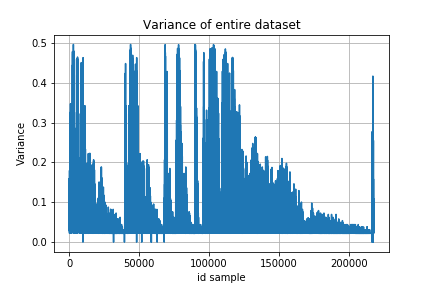
\includegraphics[width=0.6\columnwidth]{variance-all.png}
	\caption{Variance of features in the entire dataset}
	\label{fig:var_all}
\end{figure}

To remove them, we use \texttt{VarianceThreshold} class that removes all low-variance features. Is it possible to set a threshold, if a feature variance is below the threshold, then it is removed. By default, the class removes all zero-variance features. This method removes \textbf{32} features from our dataset.

\subsection{Filter methods}

Filter methods work by selecting the best features based on a ranking function. Scikit-learn offers various scoring functions, such as \textit{chi2, f\_classif, mutual\_info\_classif}. To choose the best $k$ features scikit-learn has two classes:
\begin{itemize}
	\item \texttt{SelectKBest: }removes all but the highest $k$ scoring features.
	\item \texttt{SelectPercentile} removes all but a user-specified highest scoring percentage of features.
\end{itemize} 
We use \texttt{SelectPercentile} to perform some tests with different percentages and compared the results. 
We select respectivly the 25\%, 15\%, and 10\% of the functions \texttt{chi2, fclassif, and mutual\_info} and summarized them in Figures \ref{fig:ranking} and Tables \ref{tab:rank}. The column \textit{time} in Tables \ref{tab:rank} refers to the time elapsed during the feature selection, not during the classification algorithm to test the performances.

\begin{figure}[]
	\centering
	\begin{subfigure}[t]{0.48\textwidth}
		\centering
		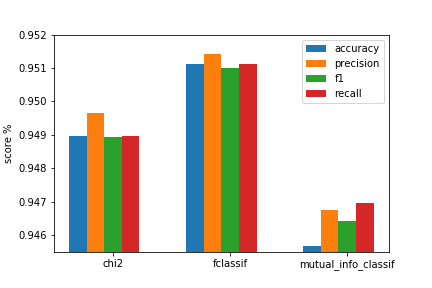
\includegraphics[width=\linewidth]{univariance25.png}
		\caption{Ranking functions score with 25\%}\label{fig:ranking25}		
	\end{subfigure}
	\begin{subfigure}[t]{0.48\textwidth}
		\centering
		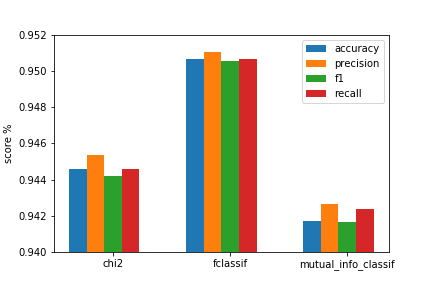
\includegraphics[width=\linewidth]{univariance15.png}
		\caption{Ranking functions score with 15\%}\label{fig:ranking15}
	\end{subfigure}\\
	\begin{subfigure}[t]{0.48\textwidth}
		\centering
		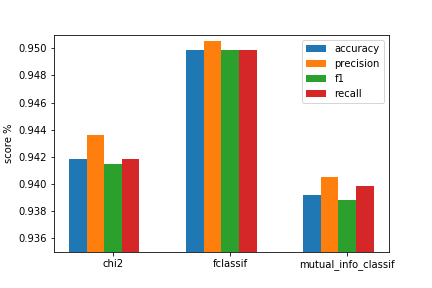
\includegraphics[width=\linewidth]{univariance10.png}
		\caption{Ranking functions score with 10\%}\label{fig:ranking10}
	\end{subfigure}
	\caption{Comparison of metrics score for different ranking functions with different percentages selected}\label{fig:ranking}
\end{figure}

As we can see from results, the \texttt{f\_classif} is the one who performs the best, even if it takes a little more time than \texttt{chi2} . On the contrary, \texttt{mutual\_info\_fclassif} is the slower, it takes half a day to calculate the mutuals information of the features, and it is also the worst in terms of performance.

However, as we reduce the percentage of features, the performances degrade too. The best percentage is 25\%, but it keeps over 50000 features, which are not good for our purpose. The classification time, instead, is acceptable, it varies from 58s for 25\% features, to 41s for 10\% features. 
We cannot rely only on filter methods because they would not shrink our dataset as we intended. So we tried other methods for feature selection provided by \textit{scikit-learn}.




\begin{table}[]

	\caption{Comparison of metrics score for different ranking functions with different percentages 	\label{tab:rank}}
	\begin{subtable}{\linewidth}
	\centering
	\caption{Summary of ranking functions selecting the 25\% of the best features}
	\label{tab:rank_function}
	\begin{tabular}{llll}
		\toprule
		\textbf{Metrics}  & \textbf{chi2} & \textbf{fclassif }& \textbf{mutual\_info} \\
		\midrule
		\texttt{Time} & 7.60s & 246.05s & 43217.97s\\
		
		\texttt{Accuracy} & 94.90\% &  95.11\% &  94.57\% \\
		\texttt{Precision}  & 94.96\% & 95.14\% &   94.67\%   \\ 
		\texttt{Recall} & 94.90\%  &   95.11\%  & 94.70\% \\ 
		\texttt{F1-score}  &   94.89\%   & 95.10\% &    94.64\%      \\ 
		\bottomrule
	\end{tabular}
	\end{subtable}

	\begin{subtable}{\linewidth}
	\centering
	\caption{Summary of ranking functions selecting the 15\% of the best features}
	\label{tab:rank_function15}
	\begin{tabular}{llll}
		\toprule
		\textbf{Metrics}  & \textbf{chi2} & \textbf{fclassif }& \textbf{mutual\_info} \\
		\midrule
		\texttt{Time} & 7.60s & 246.05s & 43217.97s\\
		
		\texttt{Accuracy} & 94.46\% &  95.06\% &  94.17\% \\
		\texttt{Precision}  & 94.54\% & 95.1\% &   94.27\%   \\ 
		\texttt{Recall} & 94.46\%  &   95.06\%  & 94.24\% \\ 
		\texttt{F1-score}  &   94.42\%   & 95.06\% &    94.17\%      \\ 
		\bottomrule
	\end{tabular}
	\end{subtable}
\begin{subtable}{\linewidth}
	\centering
	\caption{Summary of ranking functions selecting the 10\% of the best features}
	\label{tab:rank_function10}
	\begin{tabular}{llll}
		\toprule
		\textbf{Metrics}  & \textbf{chi2} & \textbf{fclassif }& \textbf{mutual\_info} \\
		\midrule
		\texttt{Time} & 7.60s & 246.05s & 43217.97s\\
		
		\texttt{Accuracy} & 94.19\% &  94.99\% &  93.92\% \\
		\texttt{Precision}  & 94.36\% & 95.05\% &   94.05\%   \\ 
		\texttt{Recall} & 94.19\%  &   94.99\%  & 93.99\% \\ 
		\texttt{F1-score}  &   94.15\%   & 94.98\% &    93.89\%      \\ 
		\bottomrule
	\end{tabular}
\end{subtable}
	
	
\end{table}


\subsection{Embedded Methods}

Embedded methods use models that have build-in feature selection methods. \texttt{RandomForestClassifier} has a field \texttt{feature\_importances} to rank all the features from best to worst. In particular, \textit{scikit-learn} provides a \texttt{SelectFromModel} class, that using a classifier that has a build-in feature importance method, select the best features based on the model. It is possible to set a \texttt{max\_features} parameter to limit the number of selected features.

However, the \texttt{SelectFromModel} algorithm chooses 12781 features in just 18s. Even with \texttt{max\_features} set to 21781 (the 10\% of the entire dataset), the algorithm still chooses only the 12781 features. Comparing the performances with the filter methods presented before, we find out that \texttt{SelectFromModel} is more accurate and the fastest in classification because there are fewer features in the feature vector. Based on those tests we prefer to discard filter methods and keep using \texttt{SelectFromModel}.

\begin{figure}[]
	\centering
	\begin{subfigure}[t]{0.48\textwidth}
		\centering
		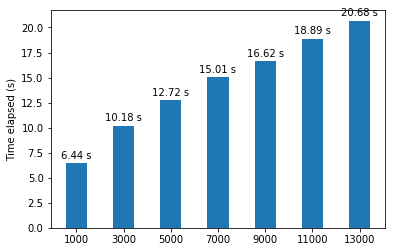
\includegraphics[width=\linewidth]{selmodel-time.png}
		\caption{Time comparison}\label{fig:model-time}		
	\end{subfigure}
	\begin{subfigure}[t]{0.48\textwidth}
		\centering
		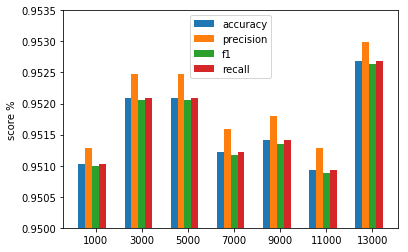
\includegraphics[width=\linewidth]{selmodel-metrics.png}
		\caption{Metrics comparison}\label{fig:model-metrics}
	\end{subfigure}
	\caption{Comparison of time and metrics score with different number of features selected using \texttt{SelectFromModel}}\label{fig:model}
\end{figure}


We run various tests with different numbers of \texttt{max	features} to compare the results. The tests are shown in Figure \ref{fig:model}. Figure \ref{fig:model-time} shows how time varies related to the number of features selected.

As we can see from Figure \ref{fig:model-metrics} there is no big difference in the tests made between \textit{accuracy, precision,recall, or f1-score}. For example, the maximum difference in accuracy is just 0.0016s. This happens because \texttt{RandomForestClassifier} already performs feature selection using \texttt{feature\_importances} during the training phase. Since the time is dependent on the number of features, we choose to balance the performances and the execution time selecting the best 3000 features.

\subsection{Wrapped methods}

As explained in Section \ref{sec:wrapper} wrapper methods are the most computational expensive. \textit{Scikit-learn} has \texttt{RFE} and \texttt{RFECV} classes for recursive feature elimination. 

From \textit{scikit-learn} documentation \cite{rfe} "\textit{The goal of recursive feature elimination (RFE) is to select features by recursively considering smaller and smaller sets of features. First, the estimator is trained on the initial set of features and the importance of each feature is obtained either through a coef\_ attribute or through a feature\_importances\_ attribute. Then, the least important features are pruned from current set of features. That procedure is recursively repeated on the pruned set until the desired number of features to select is eventually reached"}.

The \texttt{RFECV} works the same as \texttt{RFE}, but it uses a cross-validation algorithm to validate the evaluation performance.
The model used is \texttt{RandomForest} and \texttt{StratifiedKFold} as cross-validation technique.

Unfortunately, it is really slow. We tried using the entire dataset, but even after three days of computing, the algorithm didn't stop. We changed strategy, and we tried to use the features calculated from filter methods, but again it took more than three days. In the end, we decide to use the features selected by \texttt{SelctFromModel}. However, \texttt{RFECV} takes a considerable amount of time compared to other feature selection techniques.

In particular, we run tests using both the 3000 and the 1000 features selected before. As expected, the time increases exponentially with the number of features. The 3000 dataset took almost 1 hour to reduce to the optimal number of features, while the 1000 one took only 12 minutes.  Figure \ref{fig:rfecv} shows the decrease in performance as we remove more and more features from the dataset. Figure \ref{fig:rfecv-comparison} shows the comparison of evaluation metrics between the two different datasets.
Comparing the results, we did not notice a big difference in terms of accuracy precision or recall. Even if one algorithm stops at \textbf{2616} features and the other to only \textbf{842}. However, the calculation time was way longer for the first dataset. 

We continue our tests using the output of \texttt{RFECV} for 1000 features, because it was faster to calculate. 
We apply again the \texttt{SelectFromModel} algorithm to lastly reduce the number of features, leaving us with only 305 features.

\begin{figure}[]
	\centering
	\begin{subfigure}[t]{0.48\textwidth}
		\centering
		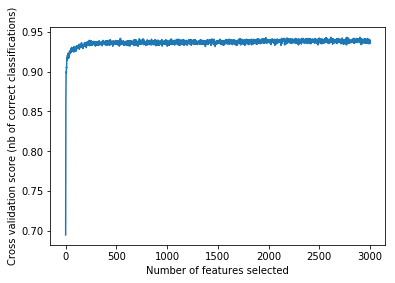
\includegraphics[width=\linewidth]{rfecv-from3000.png}
		\caption{Initial dataset contains 3000 features}\label{fig:rfecv3000}		
	\end{subfigure}
	\begin{subfigure}[t]{0.48\textwidth}
		\centering
		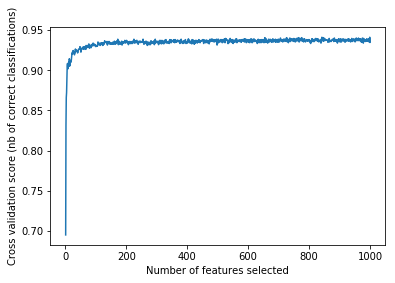
\includegraphics[width=\linewidth]{rfecv1000.png}
		\caption{Initial dataset contains 1000 features}\label{fig:rfecv1000}
	\end{subfigure}
	\caption{Relation between cross validation scores and number of features.}\label{fig:rfecv}
\end{figure}

\begin{figure}[]
	\centering
	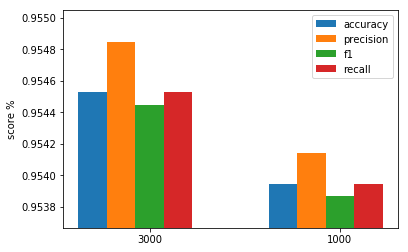
\includegraphics[width=0.6\columnwidth]{rfecv-confronto.png}
	\caption{RFECV applied respectively to a dataset of 3000, and 1000 features.}
	\label{fig:rfecv-comparison}
\end{figure}

We stopped at 305 features, because we did not notice any improvement in terms of classification time. We consider 5.5s an acceptable time for classification. Furthermore, the less features we got, the worst are the performance in evaluation, so we decide to keep that number of features.

Analyzing the type of features we have, we find that almost all the blocks of features still has some feature in the dataset. The Table \ref{tab:num-feat-842} reports the number of features keep per type. The standard library features are removed during feature selection, the others are significantly reduced.  

\begin{table}[]
	\caption{Comparison between initial number of features, and number of features after feature selection.}
	\label{tab:num-feat-842}
	\begin{tabular}{lll}
		\toprule
		Features type                    & Number & Initial number\\
		\midrule
		Disassemble Unigrams   &19 & 2476           \\
		Disassemble Bigrams    &62   & 39697          \\
		Disassemble Line Unigrams  &28& 25927          \\
		Disassemble Instruction Unigrams & 9 & 347   \\
		Disassemble Instruction Bigrams  & 19 & 8125    \\
		CFG Unigrams    &26 & 13536   \\
		CFG Bigrams      &316 & 118852  \\
		CFG Code Unigrams  & 14 & 61     \\
		CFG Code Bigrams   & 94 & 2026  \\
		CFG Complexity          & 2 & 3     \\
		Standard Library Function & 0 & 5577  \\
		Rich Header   & 4 & 1217  \\
		\bottomrule	
	\end{tabular}
\end{table}


\section{Model Evaluation}

The following section presents the tests made on the final dataset using two different models: \texttt{RandomForestClassifier} ans \texttt{XGBoostClassifier}.

We compared the results obtained with this different models, and compare them to performances of the initial dataset.

Table \ref{tab:final} summarize the executions. In the table the term \texttt{RF} means RandomForestClassifier, \texttt{XBG} means XGBoostClassifier, and \texttt{FS} means Feature Selection. To run the final tests, we chose to set  to 20 the number of repetition presented in Section \ref{sec:flow} to get a more exhaustive result.\\
The \texttt{RandomForestClassifier} is the fastest and the most accurate. With only 5s per execution, it reaches a surprisingly accuracy of 95.21\% versus the 94.76\% of \texttt{XGBoostClassifier}. Compared with the original dataset we went from more than 200 thousands features to just 304. Analyzing the performances of entire dataset and the one with feature selected, we notice that the execution time is obviously slower with the entire dataset.However,the performances metrics increased a little with our subset of relevant features.

\begin{table}[]
	\centering
	\caption{Comparison of execution time and metrics of different models}
	\label{tab:final}
	\begin{tabular}{lrcccc}
		\toprule
		\textbf{Algorithm}                          & \textbf{Time}    & \textbf{Accuracy} & \textbf{Precision} & \textbf{Recall}  & \textbf{F1-Score} \\
		\midrule
		RF with FS & 5.22s   & 95.21\%  & 95.24\%   & 95.21\% & 95.20\%  \\
		XGB with FS      & 53.14s & 94.76\%  & 94.78\%   & 94.76\% & 94.74\%  \\
		RF with full dataset   &  366.65s  & 94.98\% &       95.03\%    &   94.98\%      & 94.97\%\\
		\bottomrule         
	\end{tabular}
\end{table}
	\chapter{Future works}
\label{ch:future}
	
	\backmatter
	\cleardoublepage
	\phantomsection % Give this command only if hyperref is loaded
	\addcontentsline{toc}{chapter}{\bibname}
	
	\bibliographystyle{ieeetr}

	
	% Here put the code for the bibliography. You can use BibTeX or
	% the BibLaTeX package or the simple environment thebibliography.
	\bibliography{reference}
\end{document}